\section{Markov Chain Monte Carlo simulations}

In this problem, we are looking at a well known data set of time intervals between successive coal-mining disasters in the UK involving ten or more killed. We will adopt a Bayesian model to analyse the data and implement both a single site and a block Metropolitan-Hastings algorithm to find the underlying distribution of the parameters involved in the model. To do so we will find the posterior distribution of the underlying model parameters and the full conditional for each of the model parameters. 

\subsection{Data exploration}
To get a greater understanding of the data set, we plot it. This can be seen in Figure \ref{fig:cumul_plot}, where we have plotted the year along the x-axis and the cumulative number of disasters along the y-axis. 

\begin{figure}[h]
    \centering
    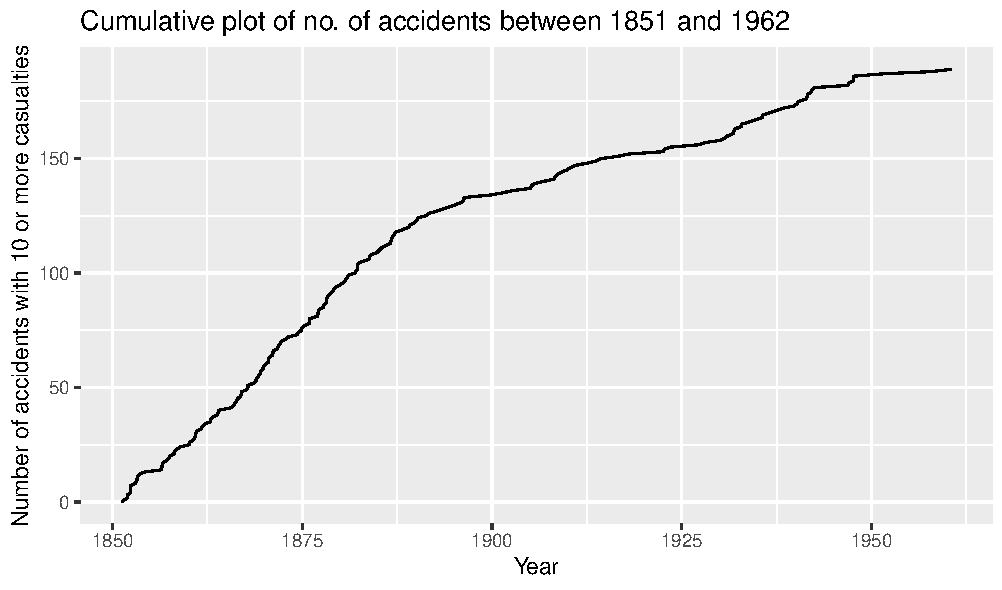
\includegraphics[width = \textwidth]{Images/cumulative_plot_data.pdf}
    \caption{Cumulative plot of coal-mining disasters in the UK occurring between 1851 and 1962.}
    \label{fig:cumul_plot}
\end{figure}

We can instantly see that the incline of the graf is different at the begining and the end of the period. It looks like this shift happens some time between 1885 and 1900. 


\subsection{Posterior distribution of underlying model parameters} \label{posterior}
%\todo[color = yellow]{Litt pirk her men når tenksten er såpass lik oppgaveteksten synes jeg der er ryddig å på en måte referere til oppgaven så det kommer tydelig fram at vi ikke har funnet det på selv. Jeg skrev det også om bittelitt}

As proposed in the exercise set we adopt a hierarchical Bayesian model to analyse the data set. We assume that the coal-mining disasters follow a inhomogeneous Poisson process with intensity function $\lambda(t)$. We assume $\lambda(t)$ to be piecewise constant with $n$ breakpoints. The start and endpoints are denoted by $t_0$ and $t_{n+1}$ for the data set and $t_k; k = 0,...,n$ denote the break points of the intensity function. In our case we only have one break point. This means,  
%\todo{Trenger jeg ha med all denne forklaringen, eller er det nok å si at n = 1 litt tidligere?} 
%\todo[color = yellow]{Forklaringen er fin men vi kan gjøre herifra og ut med våre parametre :) }

\begin{equation}
    \lambda(t) = 
    \begin{cases}
        \lambda_0 = \textbf{for } t \in [t_0,t_{1}] \text{ and }\\
        \lambda_1 = \textbf{for } t \in [t_1, t_2].
    \end{cases}
\end{equation}

The likelihood function for the observed data is given by,

\begin{align}
    f(x|t_1,\lambda_1,\lambda_2) 
    = \text{exp} \Big( - \sum_{k = 0}^1 \lambda_k (t_{k-1} - t_k) \prod_{k = 0}^1 \lambda_k^{y_k} \Big), 
\end{align}
where $x$ is the observed data and $y_k$ is the number of observed disasters in the period $t_k$ to $t_{k+1}$. 

We assume $t_1$ to be apriori uniformly distributed on $[t_0, t_2]$, and $\lambda_0, \lambda_1$ to be apriori independent of $t_1$ and of each other. We also assume $\lambda_0,\lambda_1$ to have the gamma prior distribution with $\alpha = 2$ and scale parameter $\beta$. Thus, we have 

\begin{align}
    \pi(\lambda_i | \beta) = \frac{1}{\beta^2}\lambda_i e^{-\frac{\lambda_i}{\beta}} \textbf{ for } \lambda_i \geq 0.
\end{align}

The hyper parameter $\beta$ follows the following improper distribution,

\begin{align}
    \pi (\beta) \propto \frac{\text{exp}\{ -\frac{1}{\beta} \} }{\beta} \textbf{ for } \beta > 0.
\end{align}

In total this gives us the following model parameters, $\boldsymbol{\theta} = (t_1, \lambda_0, \lambda_1, \beta)$. 
To find an expression for the posterior distribution of $\boldsymbol{\theta}$ given $x$, $f(\boldsymbol{\theta}|x)$, we use Bayes' theorem, and find that 
%\todo{forklar mer hvordan vi kommer fram til dette?}
%\todo[color = yellow]{la til mellomsteget. Det er ikke egentlig noe mer og forklare her det er sånn Bayes formula er definert :) }
\begin{align}
    f(\theta|\boldsymbol{x}) = \frac{f(\boldsymbol{x}|\theta) \pi(\theta)}{f(\boldsymbol{x})} \propto f(\boldsymbol{x}|\theta) \pi(\theta) .
\end{align}
The likelihood $f(\boldsymbol{x} | \boldsymbol{\theta})$ is given above, $\pi(\boldsymbol{\theta})$ can be computed knowing $t_1, \lambda_0$ and $\lambda_1$ are all independent. In total this means,

\begin{align}
    \pi(\boldsymbol{\theta}) 
    = \pi(t_1, \lambda_0, \lambda_1, \beta) \nonumber \\
    = \pi(t_1, \lambda_0, \lambda_1 | \beta) \cdot \pi(\beta) \nonumber \\
    = \pi(t_1) \cdot \pi(\lambda_0|\beta) \cdot \pi(\lambda_1|\beta) \cdot \pi(\beta).
\end{align}

Using this and the given likelihood, we find the posterior distribution for $f(\boldsymbol{\theta}|x)$

\begin{align} \label{eq:post}
    f(\boldsymbol{\theta}|x) \propto \text{exp} \Big( - \sum_{k = 0}^1 \lambda_k (t_{k+1} - t_k) \Big)\cdot \prod_{k = 0}^1 \lambda_k^{y_k} \cdot \frac{1}{t_2-t_0} 
    \Big( \frac{1}{\beta^2} \lambda_0 \cdot
    \text{exp} \Big({-\frac{\lambda_0}{\beta}} \Big)  \Big) \nonumber \\ 
    \cdot \Big( \frac{1}{\beta^2} \lambda_1 \cdot \text{exp} \Big({-\frac{\lambda_1}{\beta}} \Big) \Big) \cdot \text{exp} \Big( -\frac{1}{\beta} \Big)/\beta \nonumber \\
    \propto   \frac{1}{\beta^5} \cdot \lambda_0^{y_0 + 1} \cdot \lambda_1^{y_1 + 1} \cdot \text{exp} \Big( -\frac{1}{\beta}(\lambda_0 + \lambda_1 + 1) - \lambda_0(t_1-t_0) - \lambda_1(t_2-t_1) \Big)
\end{align}




%%%%%%%%%%%%%%%%%%%%%%%%%%%%%%%%%%%%%%%%%%%%%%%%%%%%%%%%%%%%%%%%%%%%%%%%%%%%%%%%%%%%%%%%%%%%%%%%%%%%%%%%%%%%%%%%%%%%%%%%%%%%%%%
\subsection{Full conditional distribution for the model parameters} \label{full_cond}

To find the full conditional for each of the elements in $\boldsymbol{\theta}$, we use the expression for the posterior distribution given in \eqref{eq:post}. When we are looking at the full conditional for one of the elements in $\boldsymbol{\theta}$ given all the others, the other parameters can be viewed as constants. This means what we can overlook them in our proportional model, and we get that the full conditional for $t_1$ is

\begin{align}
    f(t_1 | \lambda_0, \lambda_1, \beta, x) \propto 
    \lambda_0^{y_0 + 1} \lambda_1^{y_1 + 1} \cdot \text{exp} \Big( -\lambda_0(t_1 - t_0) - \lambda_1 (t_2 - t_1) \Big) \nonumber \\
    \propto  \lambda_0^{y_0 + 1} \lambda_1^{y_1 + 1} \cdot \text{exp} \Big( -(\lambda_0 - \lambda_1)t_1 \Big).
\end{align}

We do not recognize the expression for the full conditional of $t_1$ as belonging to a named distribution. 

The full conditional for $\lambda_0$ and $\lambda_1$ can also be found by using the posterior distribution given in \eqref{eq:post}. Thus, 

\begin{align}
    f(\lambda_0 | \lambda_1, t_1, \beta, x) \propto
    \lambda_0^{y_0 + 1}\cdot \text{exp} \Big( -\frac{1}{\beta} \lambda_0 - (t_1 - t_0)\lambda_0 \Big) 
    \nonumber \\
    \propto  \lambda_0^{y_0 + 1} \cdot \text{exp} \Big( - \lambda_0 (\frac{1}{\beta} + t_1 - t_0) \Big),
     \\
    f(\lambda_1 | \lambda_0, t_1, \beta, x) \propto
    \lambda_1^{y_1 + 1}\cdot \text{exp} \Big( -\frac{1}{\beta} \lambda_1 - (t_2 - t_1)\lambda_1 \Big) \nonumber \\
    \propto  \lambda_1^{y_1 + 1} \cdot \text{exp} \Big( - \lambda_1 (\frac{1}{\beta} + t_2 - t_1) \Big),
\end{align}
and we see that the full conditional for $\lambda_0$ and the full conditional for $\lambda_1$ are both gamma distributed with rate $\alpha$ and scale $\beta$ parameters respectively $\alpha_0 = y_0 + 2$, $\beta_0 = \frac{1}{\frac{1}{\beta} + t_1 - t_0}$, $\alpha_1 = y_1 + 2$, $\beta_1 = \frac{1}{\frac{1}{\beta} + t_2 - t_1}$. 



For the last parameter $\beta$, the full conditional is given by,
\begin{align}
    f(\beta | \lambda_0, \lambda_1, t_1, x) \propto 
    \frac{1}{\beta^5} \cdot \text{exp} \Big( -\frac{1}{\beta}(\lambda_0 + \lambda_1 + 1) \Big),
\end{align}

and we also recognize this as belonging to a gamma distribution with rate parameter $\alpha_{\beta} = 6$ and scale parameter $\beta_{\beta} = \frac{1}{\lambda_0 + \lambda_1 + 1} $. 

%%%%%%%%%%%%%%%%%%%%%%%%%%%%%%%%%%%%%%%%%%%%%%%%%%%%%%%%%%%%%%%%%%%%%%%%%%%%%%%%%%%%%%%%%%%%%%%%%%%%%%%%%%%%%%%

%%%%%%%%%%%%%%%%%%%%%%%%%%%%%%%%%%%%%%%%%%%%%%%%%%%%%%%%%%%%%%%%%%%%%%%%%%%%%%%%%%%%%%%%%%%%%%%%%%%%%%%%%%%%%%%


\subsection{Single site MCMC algorithm}

We have defined and implemented a single site MCMC algorithm to sample from $f(\theta |x)$ given in \ref{eq:post}. As the full conditionals of $\beta^i, \lambda_0^i$ and $\lambda_1^i$ belong to known distributions, we can use Gibbs sampling to draw directly from the full conditionals for these parameters. For $t_1$ however, this is not possible.
To find $t_1$, we use the Metropolis-Hastings step with a random walk of order one. This means we propose a new value for $t_1$ which we from now on will call $t$ from the normal distribution with the previous $t$ value as mean and a tuning parameter $\sigma$ as variance. 

%\todo[color = yellow]{Her var det noe som ikke ble helt riktig. Det som står nå er rett det som er kommentert ut er ikke helt rett}
% We draw an initial state for $t$ and then propose a new state $t_{new}$ from $Q(t_1|x)$ using a random walk step, where $Q(t_1|x)$ is our proposal distribution. We have chosen our random walk step to be normally distributed with mean $t_{old}$ and standard deviation $\sigma$.

We then compute the acceptance probability for $t_{new}$
\begin{align}
    \alpha(t_{new}|x) = \text{min} \Big( 1, \frac{f(t_{new}| \lambda_0, \lambda_1, \beta, x)}{f(t_{old}| \lambda_0, \lambda_1, \beta, x)} \Big) \nonumber \\ 
    = \text{min} \Big( \frac{\lambda_0^{y_{0_{new}} + 1} \cdot \lambda_1^{y_{1_{new}} + 1} \text{exp}(-(\lambda_0 - \lambda_1)t_{new})}{\lambda_0^{y_{0_{old}} + 1} \cdot \lambda_1^{y_{1_{old}} + 1} \text{exp}(-(\lambda_0 - \lambda_1)t_{old})} \Big) \nonumber 
\end{align}

and accept or reject the proposed $t$. We note that since the proposal density is a random walk the proposal ratio which usually is a part of the acceptance probability cancels out. Also we compute this on a log scale to avoid computational issues.

All of this gives us the following algorithm, 

%input code lines here. 
\lstinputlisting[language=R, firstline=11, lastline=87]{Code/MH_singel.R}

\subsection{Burn-in and mixing period of the algorithm}

To evaluate the burn-in period of the algorithm, we have plotted the values of $\lambda_0, \lambda_1, t_1$ and $\beta$ for $n$ iterations of our MCMC algorithm, using tuning parameter $\sigma = 10$ and starting values $\lambda_0 = 10, \lambda_1 = 5, \beta = 3$ and $t_1 = 45$. This is seen in figure \ref{fig:burnin_singleMH}. 

%\todo[color = yellow]{Husk å skrive hva vi har brukt som initialverdier og verdien til sigma}

\begin{figure}[h]
    \centering
    \begin{subfigure}[b]{0.49\textwidth}
        \centering
        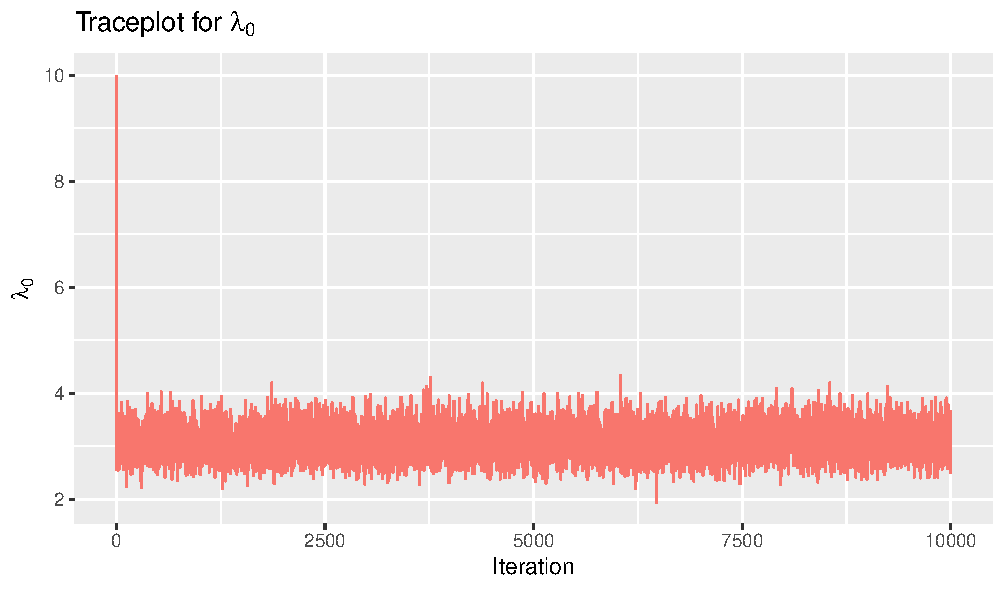
\includegraphics[width = \textwidth]{Images/sim_lambda0.pdf}
        \caption{$\lambda_0$}
        \label{fig:burnin_lam0}
    \end{subfigure}
    \begin{subfigure}[b]{0.49\textwidth}
        \centering
        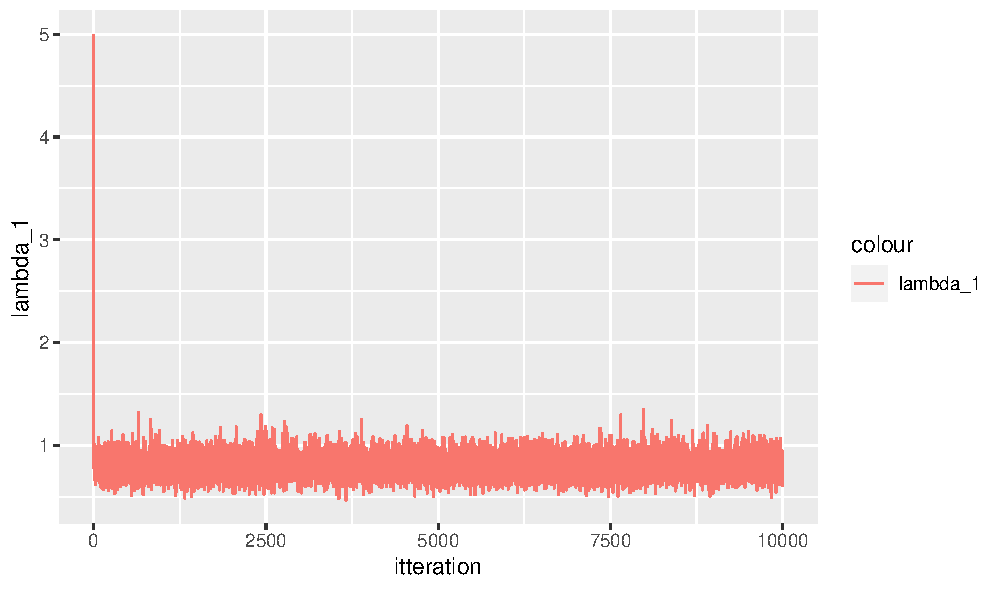
\includegraphics[width = \textwidth]{Images/sim_lambda1.pdf}
        \caption{$\lambda_1$}
        \label{fig:burnin_lam1}
    \end{subfigure}
    \begin{subfigure}[b]{0.49\textwidth}
        \centering
        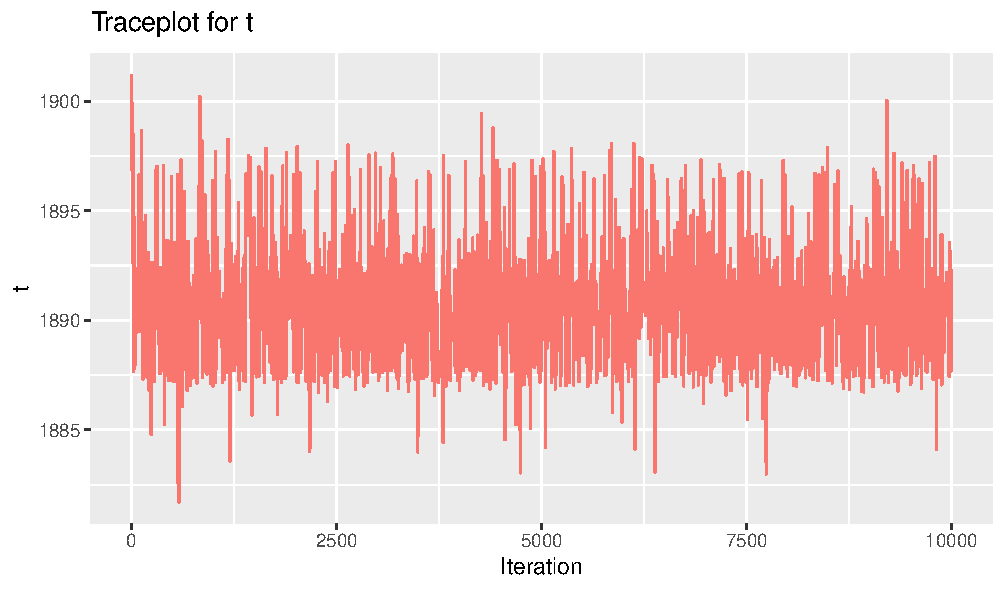
\includegraphics[width = \textwidth]{Images/sim_t.pdf}
        \caption{$t_1$}
        \label{fig:burnin_t}
    \end{subfigure}
    \begin{subfigure}[b]{0.49\textwidth}
        \centering
        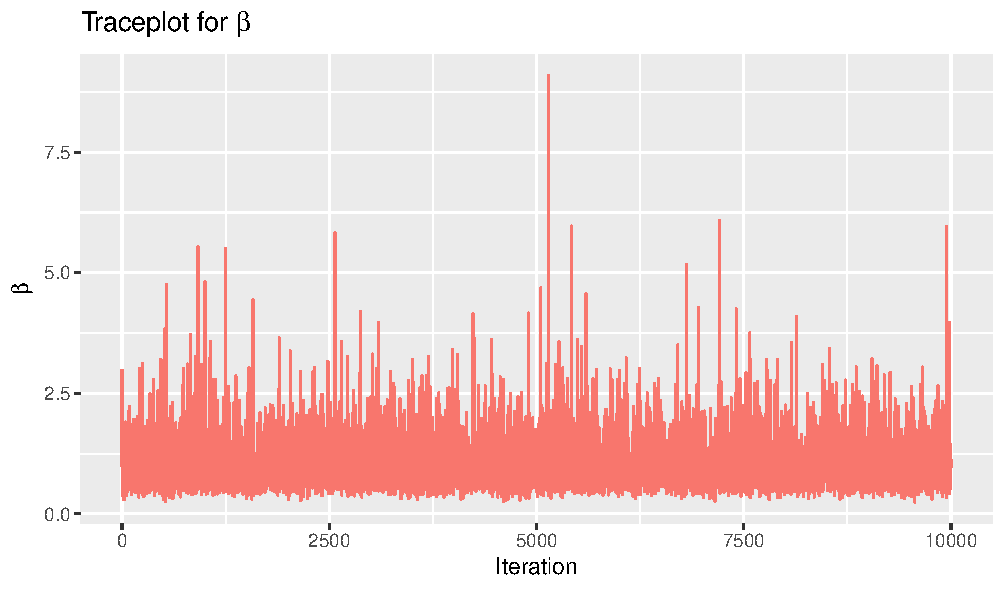
\includegraphics[width = \textwidth]{Images/sim_beta.pdf}
        \caption{$\beta$}
        \label{fig:burnin_beta}
    \end{subfigure}
    \caption{The value of $\lambda_0, \lambda_1, t_1$ and $\beta$ plotted for $n = 10000$ iterations of the MCMC algorithm. Initial values used were $\lambda_0 = 10, \lambda_1 = 5, t_1 = 45$ and $\beta = 3$. The tuning parameter used was $\sigma = 3$.}
    \label{fig:burnin_singleMH}
\end{figure}

We plotted the parameters separately so they are easier to evaluate. We need to choose a burn-in period for the algorithm equal to the longest burn-in period amongst the parameters. 
In figure \ref{fig:burnin_lam0} and \ref{fig:burnin_lam1}, we see that the simulations stabilize very quickly, and there is a very small burn-in period for these parameters. 
%\todo[inline]{burn-in for beta. Den er ikke helt stabil}
%\todo[inline]{Burn-in for t. Ikke helt stabil. Ta med plott fra forskjellige ekstremverdier av t, of forklar hvordan disse ser ut..}
For the parameter $\beta$, we see that the samples fluctuate, but the mean and variance of the simulations does not seem to change. For the $t_1$-parameter however, we see that the mean slightly changes when the number of iterations increase. 

% This means that we should investigate the burn-in period of this parameter more closely. We do this by running the algorithm for different initial values of $t$, and for different different values for the tuning parameter $\sigma$. In figure \ref{fig:sim_t_diff_start} we see the parameter $t_1$ with $n = 10000$ samples, for three different initial values of $t_1$. 

% \todo[]{Disse må kjøres på nytt, eller vent, vi trenger jo ikke disse nå som vi har mixing plottene!!!! :) :) }
% \begin{figure}[h]
%     \centering
%     \begin{subfigure}[b]{0.49\textwidth}
%         \centering
%         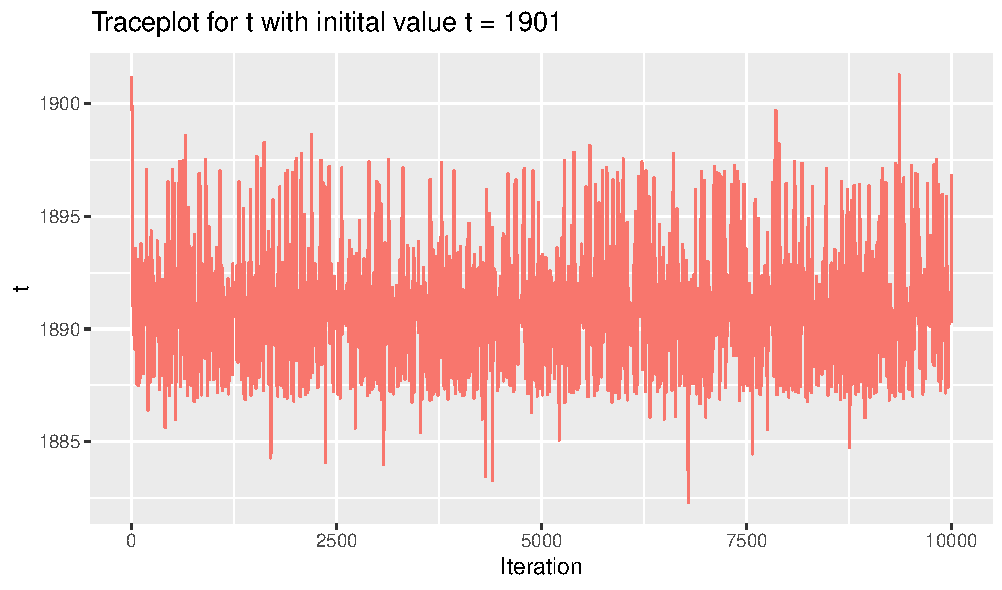
\includegraphics[width = \textwidth]{Images/sim_t_1_1.pdf}
%         \label{fig:sim_t_diff_start_35}
%     \end{subfigure}
%     \begin{subfigure}[b]{0.49\textwidth}
%         \centering
%         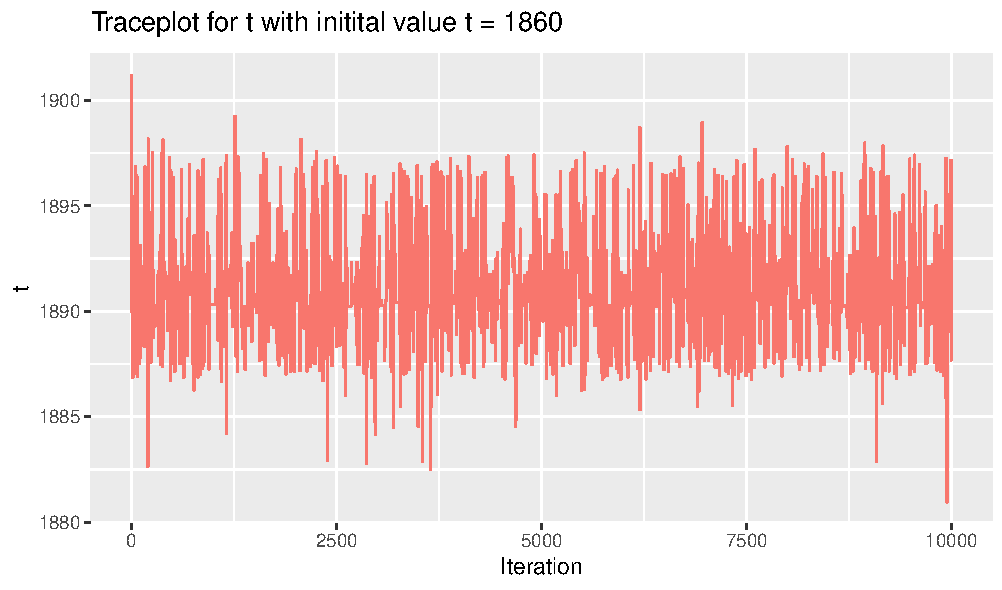
\includegraphics[width = \textwidth]{Images/sim_t_1_2.pdf}
%         \label{fig:sim_t_diff_start_45}
%     \end{subfigure}
%     \begin{subfigure}[b]{0.49\textwidth}
%         \centering
%         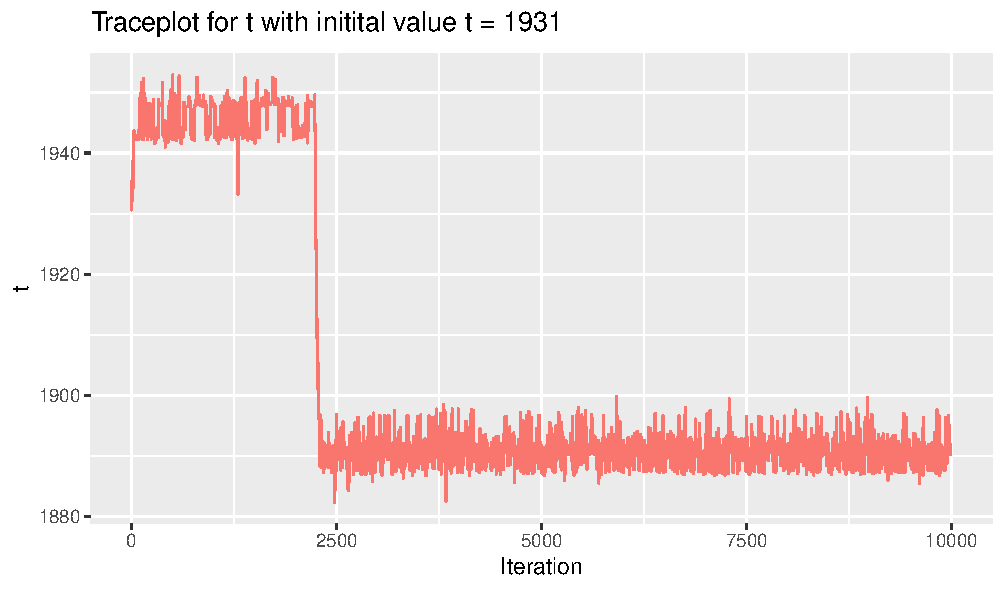
\includegraphics[width = \textwidth]{Images/sim_t_1_3.pdf}
%         \label{fig:sim_t_diff_start_90}
%     \end{subfigure}
%     \caption{Plots of $t_1$ for $n = 10000$ simulations, using different initial values for $t$.}
%     \label{fig:sim_t_diff_start}
% \end{figure}

% We see in figures \ref{fig:sim_t_diff_start} that the plots with low stating values are similar, and there is no discernible difference in the burn-in period. Both plots fluctuate a little in the first $500-1000$ samples,

% but become stable after this. In figure \ref{fig:sim_t_diff_start_90} however, when using a high initial value for $t$ we quite clearly see how a burn-in period. The first $500$ samples are clearly not converged, but once the samples come down to around $1890$, the become quite stable. This suggests a burn-in period for $t_1$ of about $500$. 


% In figure \ref{fig:sim_t_big_n}, we see the simulations of $t_1$ with $n = 50000$ and $n = 100000$ samples. 

\begin{figure}[H]
    \centering
    \begin{subfigure}[b]{0.49\textwidth}
        \centering
        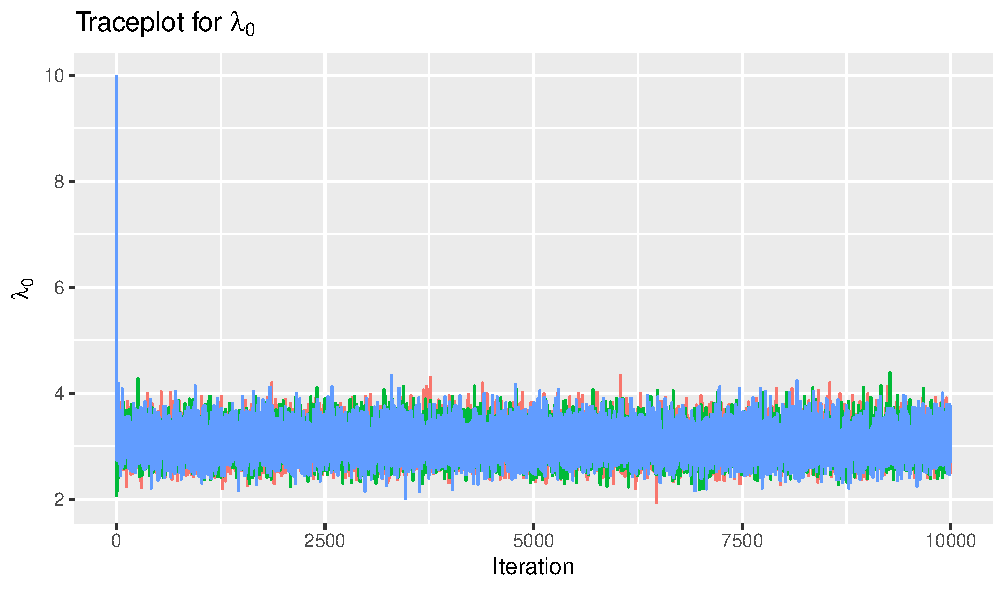
\includegraphics[width = \textwidth]{Images/mixing_lambda_0.pdf}
        \caption{$\lambda_0$ }
    \end{subfigure}
    \begin{subfigure}[b]{0.49\textwidth}
        \centering
        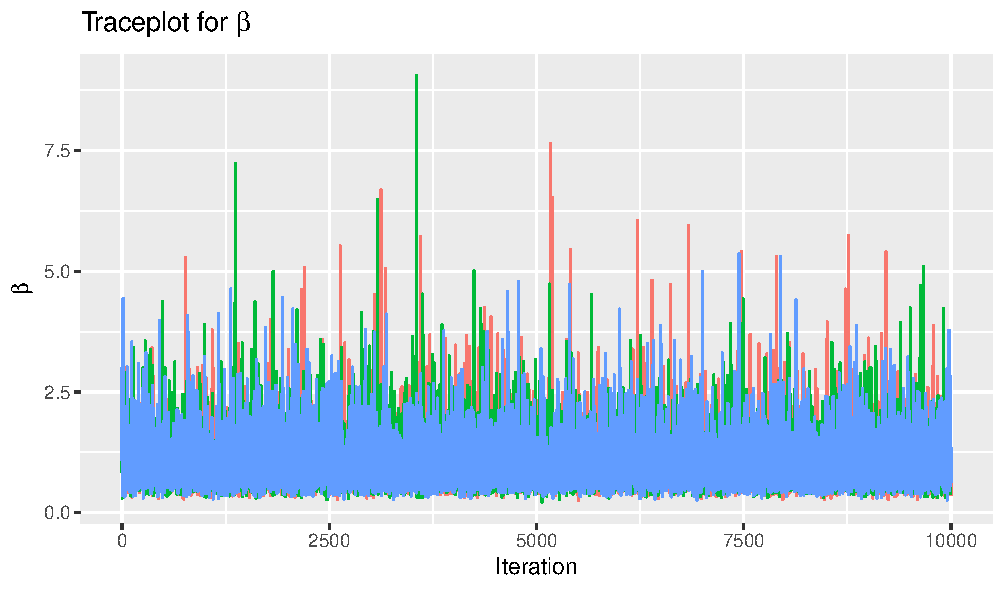
\includegraphics[width = \textwidth]{Images/mixing_lambda_1.pdf}
        \caption{$\lambda_1$}
    \end{subfigure}
    \begin{subfigure}[b]{0.49\textwidth}
        \centering
        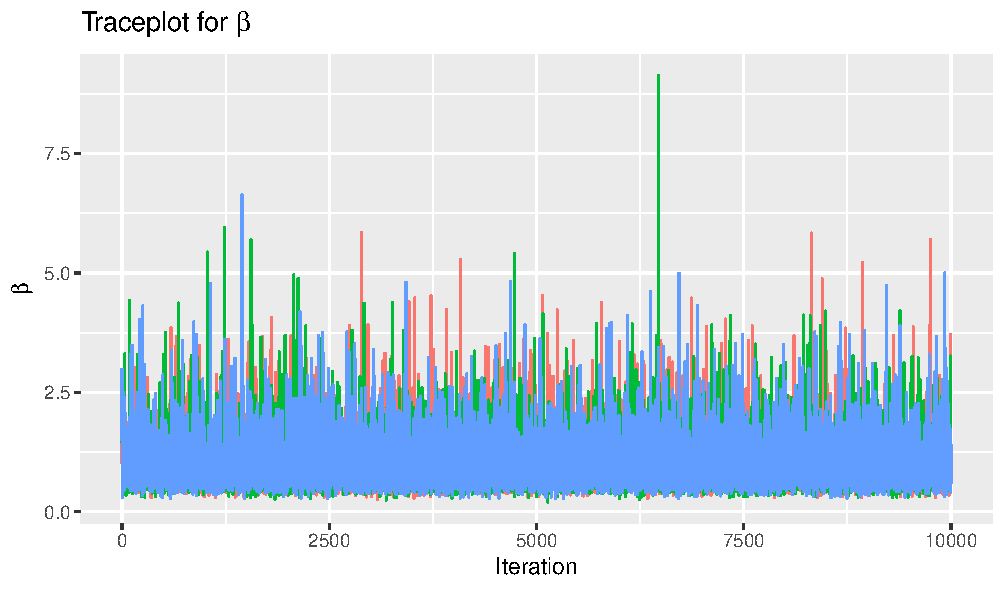
\includegraphics[width = \textwidth]{Images/mixing_beta.pdf}
        \caption{$\beta$ }
    \end{subfigure}
    \begin{subfigure}[b]{0.49\textwidth}
        \centering
        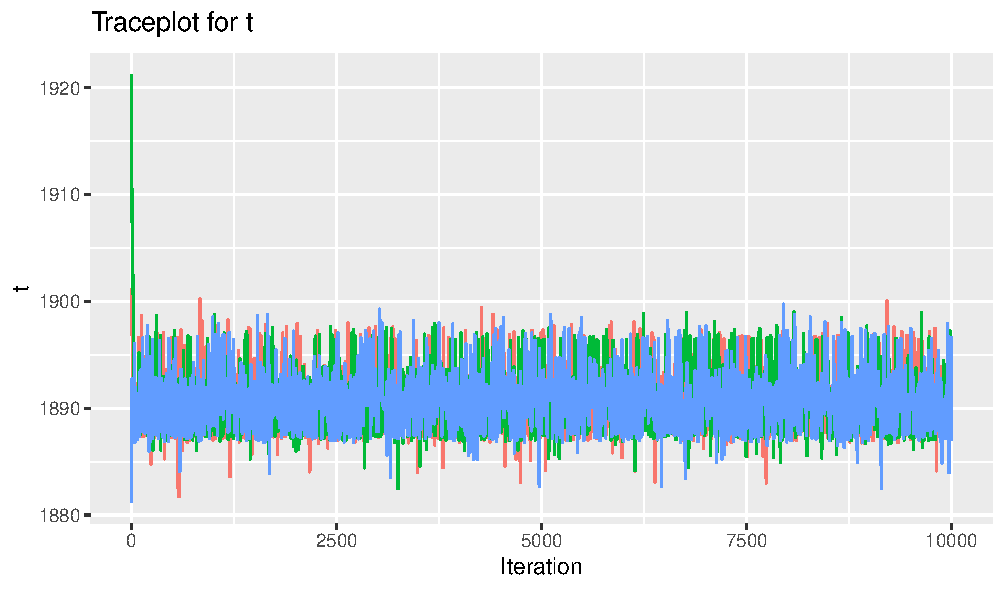
\includegraphics[width = \textwidth]{Images/mixing_t.pdf}
        \caption{$t_1$}
    \end{subfigure}
    \caption{Plot of three runs of the MCMC algorithm using $n = 10000$ simulations, using three different starting values for $t_1$.They are $t_1 = 1881$, $t_1 = 1901$ and $t = 1931$ The tuning parameter is set to $\sigma = 3$. The starting values for the other parameters are $\lambda_0 = 10, \lambda_1 = 5$ and $\beta = 3$}
    \label{fig:sim_mixing_single}
\end{figure}

% We see that the simulations of $t_1$ in figure \ref{fig:sim_t_big_n} 

%\todo[inline]{separate into two areas and calculate the statistics for the areas to evaluate if we have chosen an okay estimate for the burn-in period.}


%mixing
%\todo[color = yellow]{Dette er forsåvidt rett men ha også med et plott med to forskjellig kjeder og se hvordan de mikser}

To evaluate the burning period further we look at the mixing properties mixing properties of our algorithm, we plot three simulations of our MCMC algorithm, using three different starting values for our parameter $t_1$. As this was where we saw was the most critical for the burn in period. This should ideally be done for many different combinations ot all parameters but since we only have a limited amount of time for this project we chose to focus on $t$. The plot of the mixing for all parameters can be seen in figure .... We see in figure ... that the plots with different starting values of $t_1$ converges quite quickly, and can therefore assume that the mixing is fast. 

To further investigate the mixing properties of $t_1$, we plotted the autocorrelation function for $t_1$ after the initial burn-in period, which we have set to be $b = 500$ iterations. The autocorrelation plot is shown in figure \ref{fig:acf_t}. From the plot we see that the correlation decreases between the samples as the distance increases, and after $lag = 20$, there is no significant autocorrelation between the drawn samples. This indicates that correlation between the samples decrease fast enough for the algorithm to explore the density properly. 

\todo[color = yellow]{ACF plottet må genererers på nytt :) Skal bare være å kjøre scriptet så må du lagre acf plottet sånn du gjøre det }
\begin{figure}[H]
    \centering
    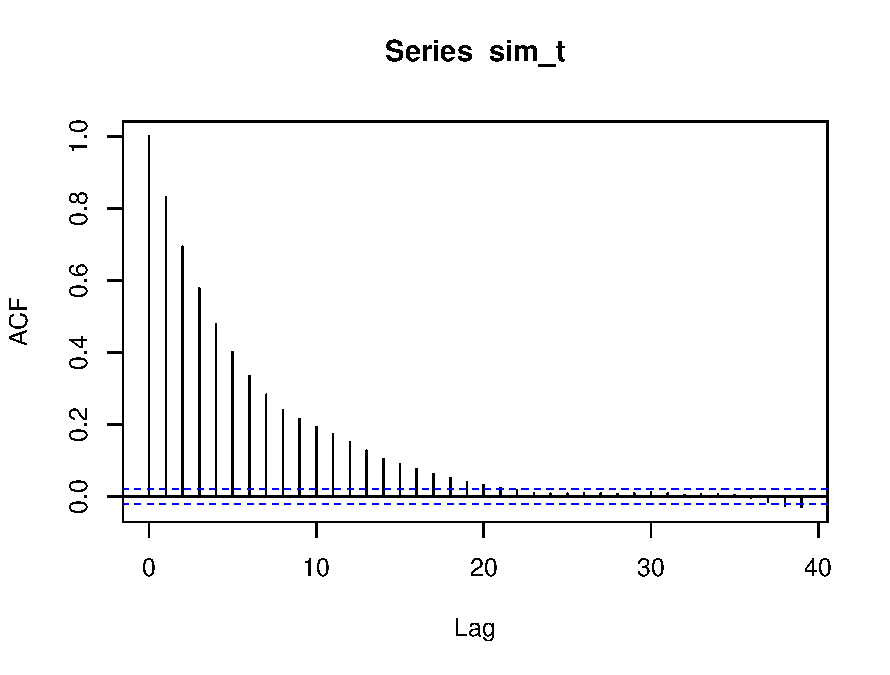
\includegraphics[width = \textwidth]{Images/acf_t_10000.pdf}
    \caption{Autocorrelation function of $t_1$ for different $lag$. }
    \label{fig:acf_t}
\end{figure}

To investigate whether the parameters estimated from the MCMC algorithm seem reasonable, we again discard the burn-in period, and then look at the mean values of the parameters after this. Our estimates are then $\lambda_0 = 3.081, \lambda_1 = 0.927 , \beta = 1.004 $ and $t_1 = 1891$. Looking at figure \ref{fig:gaussian_data}, we see that the rate of registered accidents changes around year $1890$, which is consistent with the estimated $t_1$. The total number of accidents registered in the data set is $189$. This means that our parameter estimates should give a similar number of total accidents. We have that
\begin{align}
    \text{Total no. of accidents} = \lambda_0(t_1 - t_0) + \lambda_1(t_2 - t_1) \nonumber \\
    = 3.081*(1891-1851.203) + 0.927*(1962.22 - 1891) = 189.04, 
\end{align}

which indicates that the estimates for $\lambda_0, \lambda_1$ and $t_1$ are reasonable. ..



%%%%%%%%%%%%%%%%%%%%%%%%%%%%%%%%%%%%%%%%%%%%%%%%%%%%%%%%%%%%%%%%%%%%%%%%%%%%%%%%%%%%%%%%%%%%%%%%%%%%%%%%%%%%%%%%%%%%%%%%%%%%%%%

%%%%%%%%%%%%%%%%%%%%%%%%%%%%%%%%%%%%%%%%%%%%%%%%%%%%%%%%%%%%%%%%%%%%%%%%%%%%%%%%%%%%%%%%%%%%%%%%%%%%%%%%%%%%%%%%%%%%%%%%%%%%%%%
\subsection{The tuning parameter and how it influences the burn-in and mixing of the simulated Markov Chain}

\begin{figure}[h]
    \centering
    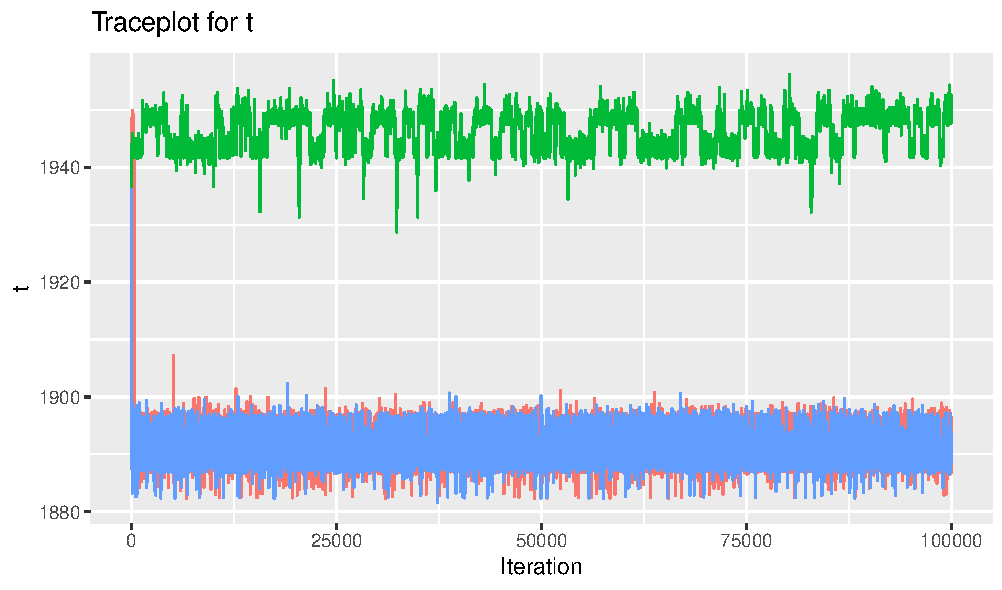
\includegraphics[width = \textwidth]{Images/tuning_stuck_t.pdf}
    \caption{Simulations of $t_1$ with different values for the tuning parameter $\sigma$, for $n = 10000$ samples. Initial values used were $\lambda_0 = 10, \lambda_1 = 5, \beta = 3$ and $t_1 = 1931$.  $\sigma = 1$,  $\sigma= 10$,  $\sigma= 20$}
    \label{fig:tuning_t_single}
\end{figure}

We have implemented our Markov Chain Monte Carlo algorithm with a tuning parameter $\sigma$. The tuning parameter is the variance for our proposal distribution $Q()$. For our parameter $t$, the tuning parameter will change the acceptance rate of the algorithm. By using a small tuning parameter $\sigma$, the new proposal $t_{new}$ will be similar to the old value $t_{old}$ and the mixing will be slow. When increasing the tuning parameter, the variance in the proposal distribution is increased, and $t_{new}$ will vary more from $t_{old}$. This means that correlation between the samples decreases and the mixing increases. We can adjust the tuning parameter such that we get enough mixing for the algorithm to take large enough steps to explore the target density efficiently, but not so large that the acceptance rate becomes too low. We are looking for an acceptance rate of $20 - 50\%$. In figure \ref{fig:tuning_t_single} we can see how the tuning parameter $\sigma$ affects the simulated samples of $t$.  In Figure \ref{fig:tuning_t_single} we used $sigma_1 = 10$, $sigma_2 = 1$ and $sigma_3 = 20$. Here we see that with the smallest $\sigma$ the algorithm gets stuck in a local maximum. The hole density is not explored within this amount of iterations. This again leads to a very large burn-in period. For the larger values of $\sigma$ the convergence seems to happen very fast. 
In Figure \ref{fig:tuning_t_single_2} we can see that for a slightly higher low value for $\sigma$ it is stuck in the same way to begin with but converges eventually.

\begin{figure}[H]
    \centering
    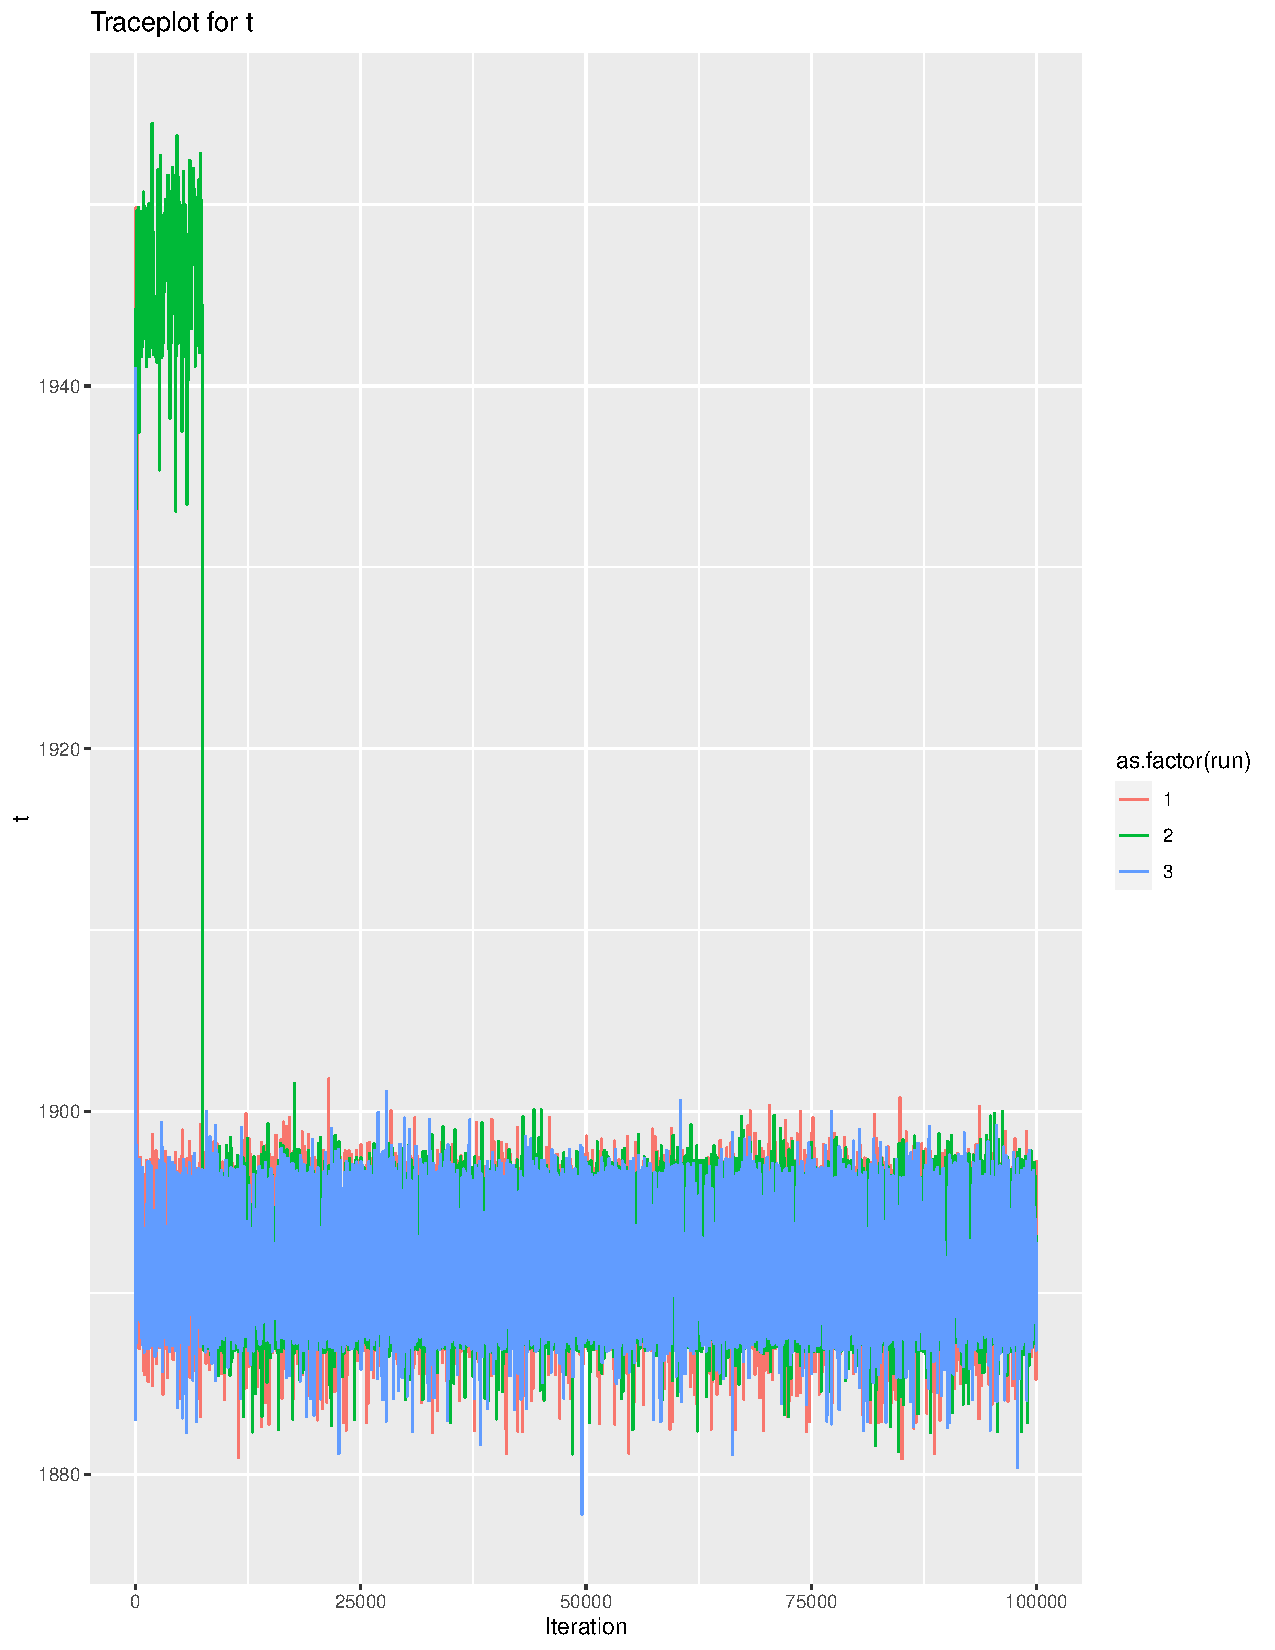
\includegraphics[width = \textwidth]{Images/tuning_t_nice.pdf}
    \caption{Simulations of $t_1$ with different values for the tuning parameter $\sigma$, for $n = 10000$ samples. Initial values used were $\lambda_0 = 10, \lambda_1 = 5, \beta = 3$ and $t_1 = 1931$. $\sigma = 2$,  $\sigma= 10$,  $\sigma= 20$}
    \label{fig:tuning_t_single_2}
\end{figure}


%%%%%%%%%%%%%%%%%%%%%%%%%%%%%%%%%%%%%%%%%%%%%%%%%%%%%%%%%%%%%%%%%%%%%%%%%%%%%%%%%%%%%%%%%%%%%%%%%%%%%%%%%%%%%%%%%%%%%%%%%%%%%%%

%%%%%%%%%%%%%%%%%%%%%%%%%%%%%%%%%%%%%%%%%%%%%%%%%%%%%%%%%%%%%%%%%%%%%%%%%%%%%%%%%%%%%%%%%%%%%%%%%%%%%%%%%%%%%%%%%%%%%%%%%%%%%%%
\subsection{Implementing a block Metropolis-Hastings algorithm}

To improve the performance of our Metropolis-Hastings algorithm, we try to perform blocking of the parameters. This means that not all parameters in $\theta$ are treated individually. Grouping together certain parameters in $\theta$ may be useful when they are correlated. We will then compute the acceptance probability, and either update all parameters within the block or none of them. We will implement a block Metropolis-Hastings algorithm with two blocks. This should have been done one a log scale to avoid computational errors. This however we did not get to work while we did get it to work not using the log scale. 

%A block Metropolis-Hastings algorithm for $f(\theta|x)$ can be defined as 
%skriv noe om Gibbs sampling?

We alternate between blocking together $t_1, \lambda_0$ and  $ \lambda_1$ and keeping $\beta$ unchanged, and blocking $\beta, \lambda_0$ and $\lambda_1$ together, keeping $t_1$ unchanged.


\subsubsection{Using a block proposal for $(t_1, \lambda_0, \lambda_1)$ keeping $\beta$ unchanged}

For the first block proposal, our target distribution is

\begin{align}
    f(t_1, \lambda_0, \lambda_1|\beta, x) = \text{exp} \Big( -(t_1-t_0)\lambda_0 -(t_2-t_1)\lambda_1 - \frac{1}{\beta}(\lambda_0 - \lambda_1)\Big) \cdot\lambda_0^{y_0 + 1} \cdot \lambda_1^{y_1 + 1}.
\end{align}

% Proposal distribution. Skriv om RW
We use Metropolis Hastings with a random walk of order one, and the random walk proposal values are generated by firstly generating $\widetilde{t_1}$ from a normal distribution, and then using the value for $\widetilde{t_1}$ when generating ($\widetilde{\lambda_0}$, $\widetilde{\lambda_1}$) from their joint full conditional. This is then used as the proposal function. As we assume $\lambda_0$ and $\lambda_1$ independent, we have that 

\begin{align}
    Q(\widetilde{t_1}, \lambda_0, \lambda_1 |t, x, \beta) = f(\lambda_0| \lambda_1, x, \widetilde{t_1}, \beta)\cdot f(\lambda_1| \lambda_0, x, \widetilde{t_1}, \beta)\cdot f(\widetilde{t_1}| t) 
    %\\
    % = \lambda_0^{y_0 + 1} \cdot \lambda_1^{y_1 + 1} \cdot \text{exp} \Big(  -\lambda_0(\frac{1}{\beta} + \widetilde{t_1} - t_0) - \lambda_1(\frac{1}{\beta} + t_2 - \widetilde{t_1})  \Big)  \nonumber \\ \cdot \frac{1}{\sqrt{2 \pi}\sigma_t } \cdot exp \Big(  -\frac{1}{2} \frac{(\widetilde{t_1}-t_1)^2}{\sigma_t^2} \Big).
\end{align}
%\todo[color = yellow]{Vi trenger ikke skrive ut det fulle uttrukket, det over holder. I tillegg er det som er kommentert ut ikke helt riktig husk at lamdaene også har nye og gamele verdier så nesten ingen ting kanselerer}

For the acceptance probability, we have that

%Acceptance probability
\begin{align}
    \alpha = \text{min} \Bigg(1,  \frac{
    f(t_{new}, \lambda_{0_{new}}, \lambda_{1_{new}}|\beta, x)}{f(t_{old}, \lambda_{0_{old}}, \lambda_{1_{old}}|\beta, x)}
    \cdot 
    \frac{Q(t_{old}, \lambda_{0_{old}}, \lambda_{0_{old}} | \beta, x, t_{new})}{Q(t_{new}, \lambda_{0_{new}}, \lambda_{0_{new}} | \beta, x, t_{old})} \Bigg) 
\end{align}



%%%%%%%%%%%%%%%%%%%%%%%%%%%%%%%%%%%%%%%%%%%%

%%%%%%%%%%%%%%%%%%%%%%%%%%%%%%%%%%%%%%%%%

\subsubsection{Using a block proposal for $\beta, \lambda_0, \lambda_1$ keeping $t_1$ unchanged}

To generate a block proposal for $\beta, \lambda_0, \lambda_1$ keeping $t_1$ unchanged, we have a target distribution which is 

\begin{align}
    f(\beta, \lambda_0, \lambda_1| t_1, x) = 
    \lambda_0^{y_0 + 1} \cdot \lambda_1^{y_1 + 1} \cdot \frac{1}{\beta^5} \cdot \text{exp}\Bigg(  -\lambda_0(t_1 - t_2) 
    - \lambda_1 (t_2 - t_1 ) 
    - \frac{1}{\beta} \cdot (\lambda_0 + \lambda_1  + 1) \Bigg). 
\end{align}

%Proposal distribution

Again, we choose to have a random walk as our proposal density. Now, we generate the potential values by first generating $\widetilde{\beta}$ from a normal distribution, this being the random walk, and then and then generating ($\widetilde{\lambda}_0, \widetilde{\lambda}_1$) from their resulting joint conditional using $\widetilde{\beta}$, $f(\lambda_0, \lambda_1|x,t_1,\widetilde{\beta})$. 
We again consider $\lambda_0$ and $\lambda_1$ independent, so the joint conditional is just the full conditionals of each multiplied. We can then find an expression for the proposal function,

\begin{align}
    Q(\widetilde{\beta}, \lambda_0, \lambda_1| \beta, t, x) = f(\lambda_0| \lambda_1, x, \widetilde{\beta}, t_1)\cdot f(\lambda_1| \lambda_0, x, \widetilde{\beta}, t_1)\cdot f(\widetilde{\beta}| \beta) 
\end{align}



%Acceptance probability

For the acceptance probability, we then have that 

\begin{align}
    \alpha = \text{min} \Bigg(1,  \frac{
    f(\beta_{new}, \lambda_{0_{new}}, \lambda_{1_{new}}|t_1, x)}{f(\beta_{old}, \lambda_{0_{old}}, \lambda_{1_{old}}|t_1, x)}
    \cdot 
    \frac{Q(\beta_{old}, \lambda_{0_{old}}, \lambda_{0_{old}} | t_1, x, \beta_{new})}{Q(\beta_{new}, \lambda_{0_{new}}, \lambda_{0_{new}} | t_1, x, \beta_{old})} \Bigg) %\\
    % = min \Bigg(1, \frac{ exp \Big( -\lambda_0 \beta_{new} +\lambda_1 \beta_{new}  \Big)}{ exp \Big( -\lambda_0 \beta_{old} +\lambda_1 \beta_{old} \Big)} 
    % \cdot \frac{ exp \Big(  -\lambda_0 \beta_{new} + \lambda_1 \beta_{new}  -\frac{1}{2} \frac{(\widetilde{\beta}_{new}-\beta_{new})^2}{\sigma_{\beta}^2} \Big)}{ exp \Big(  -\lambda_0 \beta_{old}  + \lambda_1 \beta_{old}  -\frac{1}{2} \frac{(\widetilde{\beta}_{old}-\beta_{old})^2}{\sigma_{\beta}^2} \Big)}  \Bigg).
\end{align}

%\todo[color = yellow]{Se kommentaren over}


%input the code for the algorithm. Remember to clean the code for all print statements. 

First we code all target and proposal distributions needed.
\lstinputlisting[language=R, firstline=19, lastline=111]{Code/MH_block.R}

Then we code the actual algorithm
\lstinputlisting[language=R, firstline=113, lastline=270]{Code/MH_block.R}

The trace plots for the MCMC-algorithm with block Metropolis-Hastings steps are shown in figure \ref{fig:burnin_blockMH}. 

\begin{figure}[H]
    \centering
    \begin{subfigure}[b]{0.45\textwidth}
        \centering
        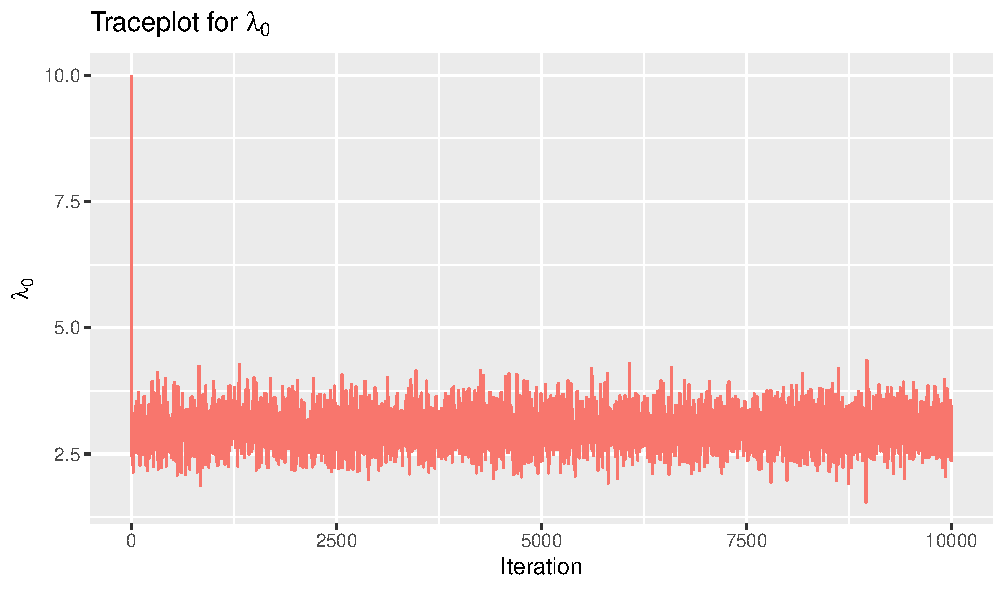
\includegraphics[width = \textwidth]{Images/block_sim_lambda0.pdf}
        \caption{$\lambda_0$}
    \end{subfigure}
    \begin{subfigure}[b]{0.45\textwidth}
        \centering
        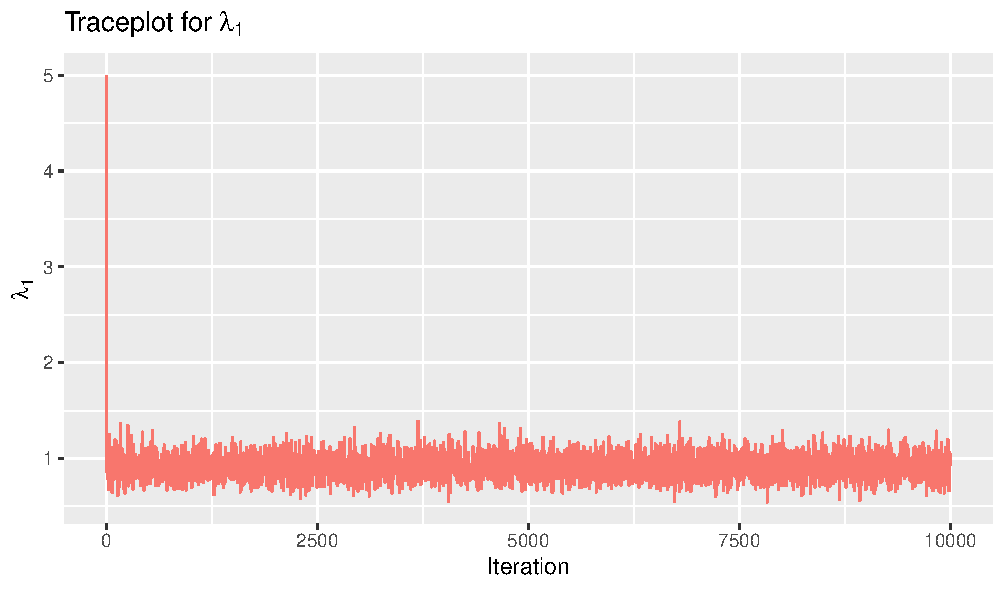
\includegraphics[width = \textwidth]{Images/block_sim_lambda1.pdf}
        \caption{$\lambda_1$}
    \end{subfigure}
    \begin{subfigure}[b]{0.45\textwidth}
        \centering
        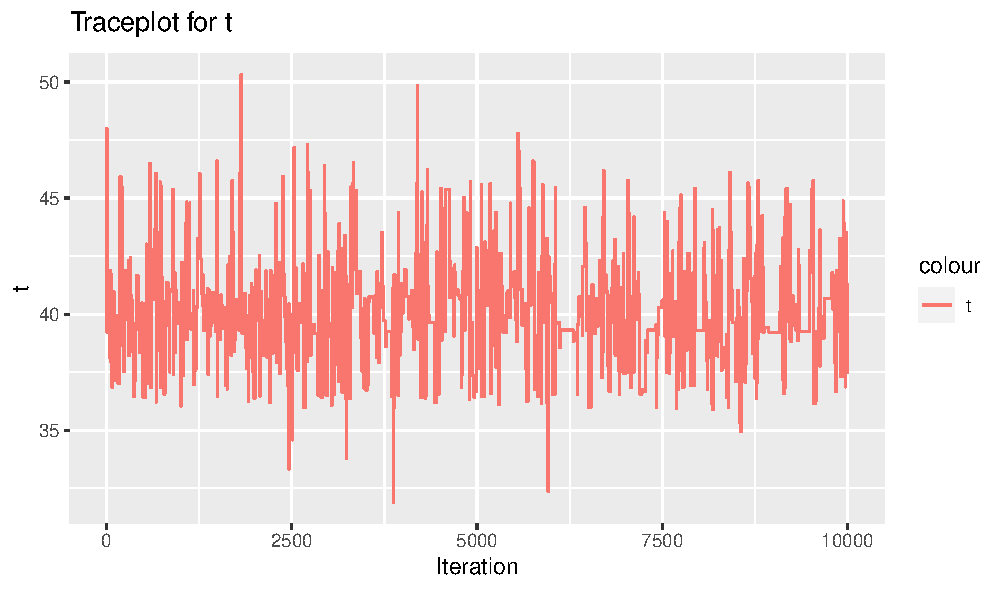
\includegraphics[width = \textwidth]{Images/block_sim_t_sigma10.pdf}
        \caption{$t_1$}
    \end{subfigure}
    \begin{subfigure}[b]{0.45\textwidth}
        \centering
        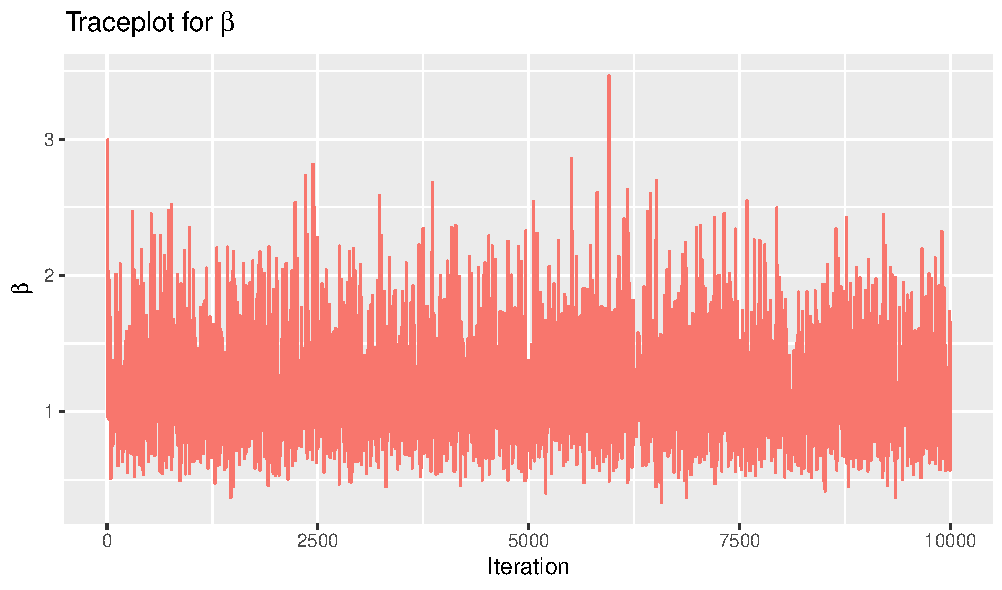
\includegraphics[width = \textwidth]{Images/block_sim_beta_sigma1.pdf}
        \caption{$\beta$}
    \end{subfigure}
    \caption{Trace plots for $n = 10000$ simulations of the different parameters with the block MCMC algorithm. The initial values used are the same as for single site MCMC, namely $\lambda_0 = 10, \lambda_1 = 5, \beta = 3$ and $t_1 = 1901$, and the tuning parameters used are $\sigma_t = 10$ and $\sigma_{\beta} = 1$}
    \label{fig:burnin_blockMH}
\end{figure}

We can see from figure \ref{fig:burnin_blockMH} that all of the parameters seem to converge quite rapidly. 
Nevertheless we try and run it for different starting values for both $t$ and $\beta$.

\subsection{The block Metropolitan-Hastings algorithm for different starting values}

\begin{figure}[H]
    \centering
    \begin{subfigure}[b]{0.49\textwidth}
        \centering
        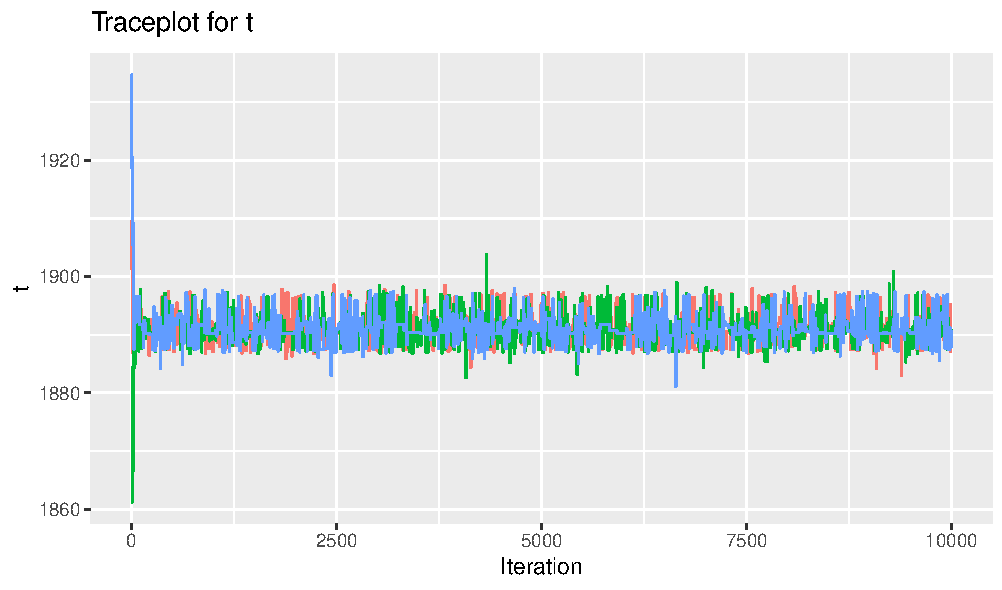
\includegraphics[width = \textwidth]{Images/mixing_t_block.pdf}
        \caption{$t$}

    \end{subfigure}
    \begin{subfigure}[b]{0.49\textwidth}
        \centering
        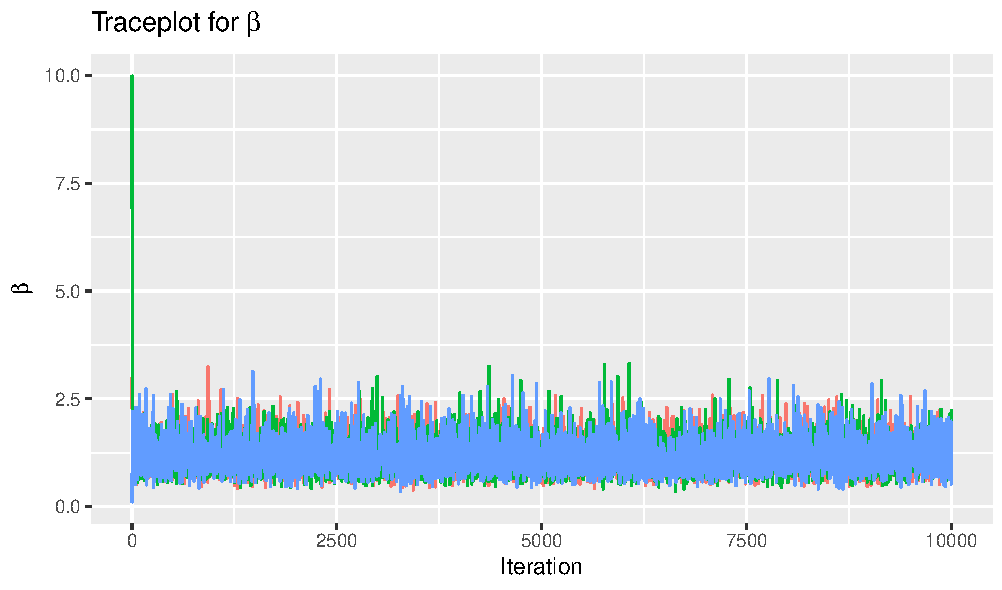
\includegraphics[width = \textwidth]{Images/mixing_beta_block.pdf}
        \caption{$\beta$}

    \end{subfigure}
    \begin{subfigure}[b]{0.49\textwidth}
        \centering
        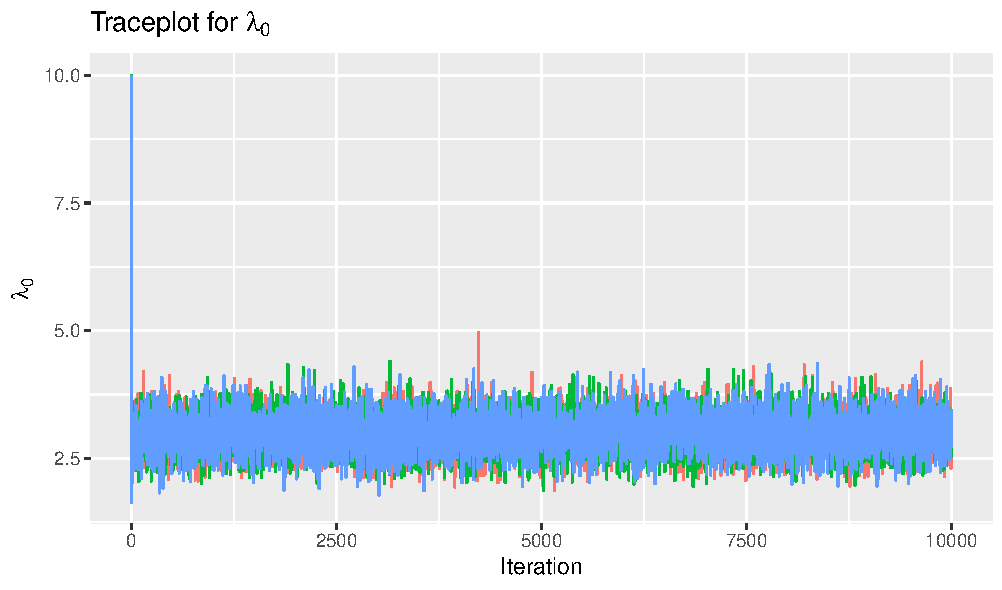
\includegraphics[width = \textwidth]{Images/mixing_lambda_0_block.pdf}
        \caption{$\lambda_0$}

    \end{subfigure}
    \begin{subfigure}[b]{0.49\textwidth}
        \centering
        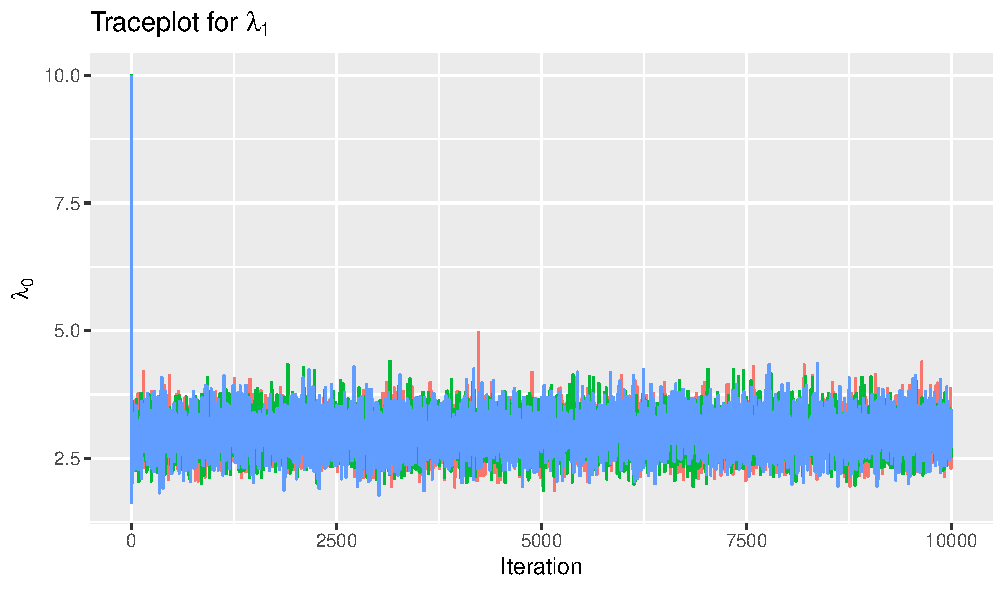
\includegraphics[width = \textwidth]{Images/mixing_lambda_1_block.pdf}
        \caption{$\lambda_1$}

    \end{subfigure}
    \caption{Trace plots for $n = 10000$ simulations of the different parameters with the block MCMC algorithm. The initial values used are $\lambda_0 = 10, \lambda_1 = 5$. For $t$ and $\beta$ we use (1901, 3), (1861, 10) and (1931, 0.1) }
    \label{fig:mixing_blockMH}
\end{figure}


We can se from Figure \ref{fig:mixing_blockMH} that the chanes mix well and it is almost imposible to distinguishe them from one another. This suggests good mixing properties. 


\subsection{The block Metropolitan-Hastings algorithm for different values of the tuning parameter}

In the block Metropolis-Hastings algorithm, we have two different tuning parameters. One for each of the different block proposals. 

The different block proposals does not run completely independently of each other, as the values proposed in one block is used in the other block if accepted. Optimaly we would tune this using a grid. But since this is quite time consuming we first look at 3 different values for $\sigma_t$ before looking at three different values for $\sigma_{\beta}$.
% However, as only one of the tuning parameters are used at a time, one in each block, the tuning parameter for each block will not significantly change the trace plot for the parameter updated in the other block. Because of this, we have chosen to change the tuning parameters separately, and then see how this change changes mixing and the acceptance rates for proposals of the parameter in that block. 



\begin{figure}[H]
    \centering
    \begin{subfigure}[b]{0.49\textwidth}
        \centering
        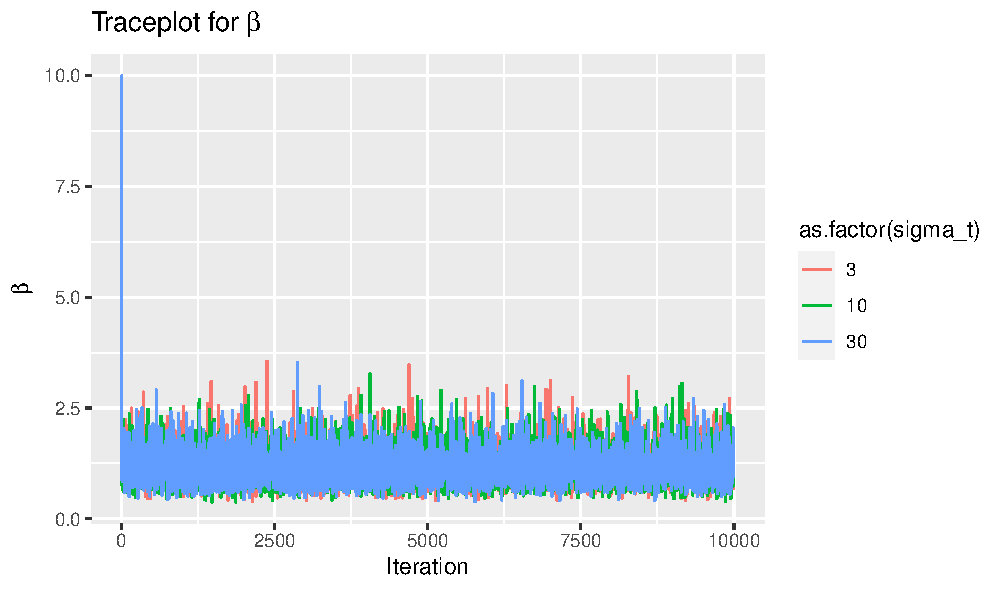
\includegraphics[width = \textwidth]{Images/tuning_beta_block.pdf}
        \caption{$\beta$}

    \end{subfigure}
    \begin{subfigure}[b]{0.49\textwidth}
        \centering
        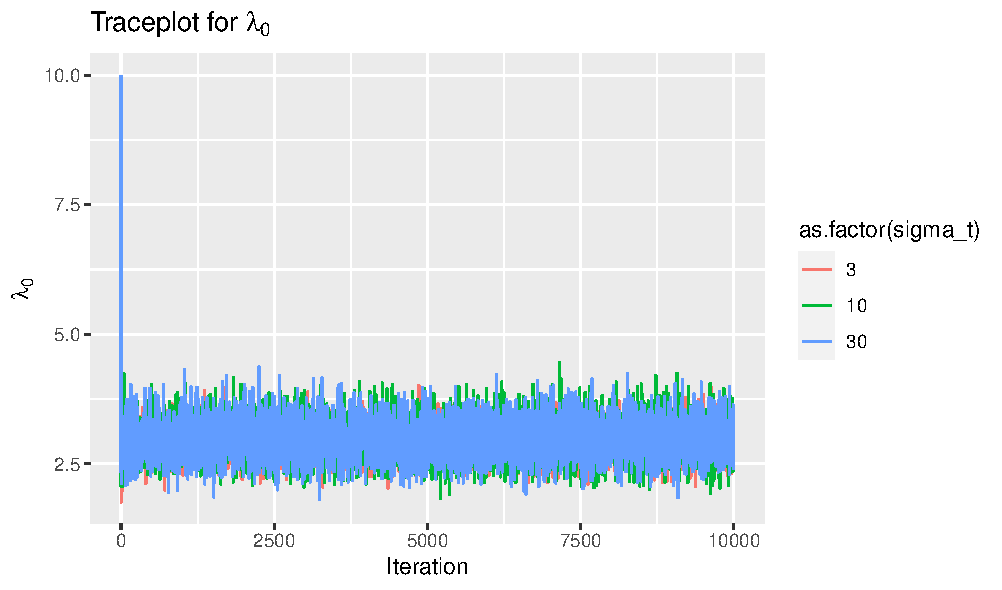
\includegraphics[width = \textwidth]{Images/tuning_lambda_0_block.pdf}
        \caption{$\lambda_0$}

    \end{subfigure}
    \begin{subfigure}[b]{0.49\textwidth}
        \centering
        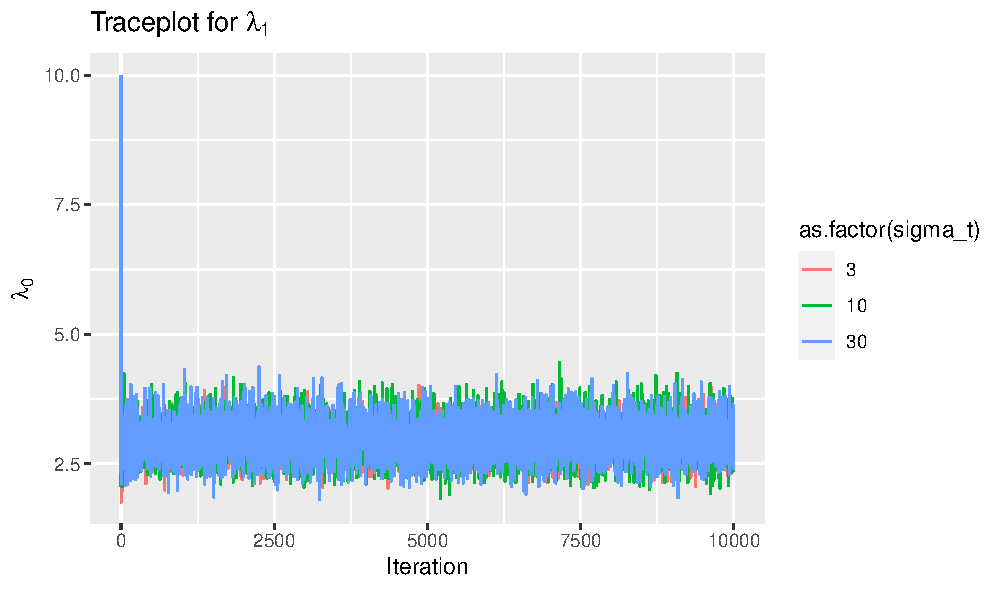
\includegraphics[width = \textwidth]{Images/tuning_lambda_1_block.pdf}
        \caption{$\lambda_1$}

    \end{subfigure}
    \begin{subfigure}[b]{0.49\textwidth}
        \centering
        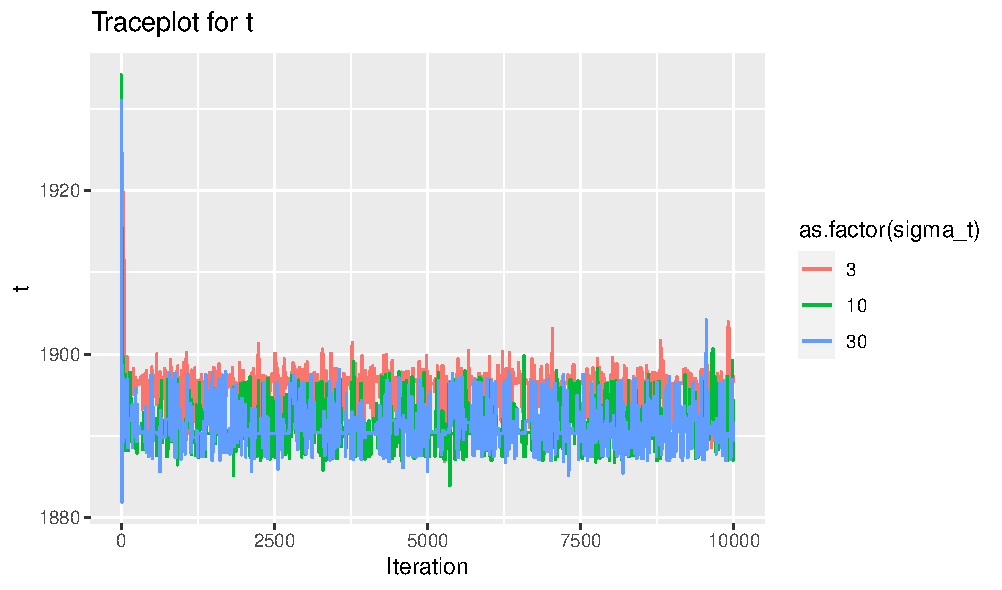
\includegraphics[width = \textwidth]{Images/tuning_t_block.pdf}
        \caption{$t$}

    \end{subfigure}
    \caption{Trace plots for $n = 10000$ simulations of the different values for $\sigma_t$ with the block MCMC algorithm. The initial values used are $\lambda_0 = 10, \lambda_1 = 5$ and $beta = 1$. For $t$ we use (3, 10, 30) }
    \label{fig:tuning_t_blockMH}
\end{figure}

\begin{figure}[H]
    \centering
    \begin{subfigure}[b]{0.49\textwidth}
        \centering
        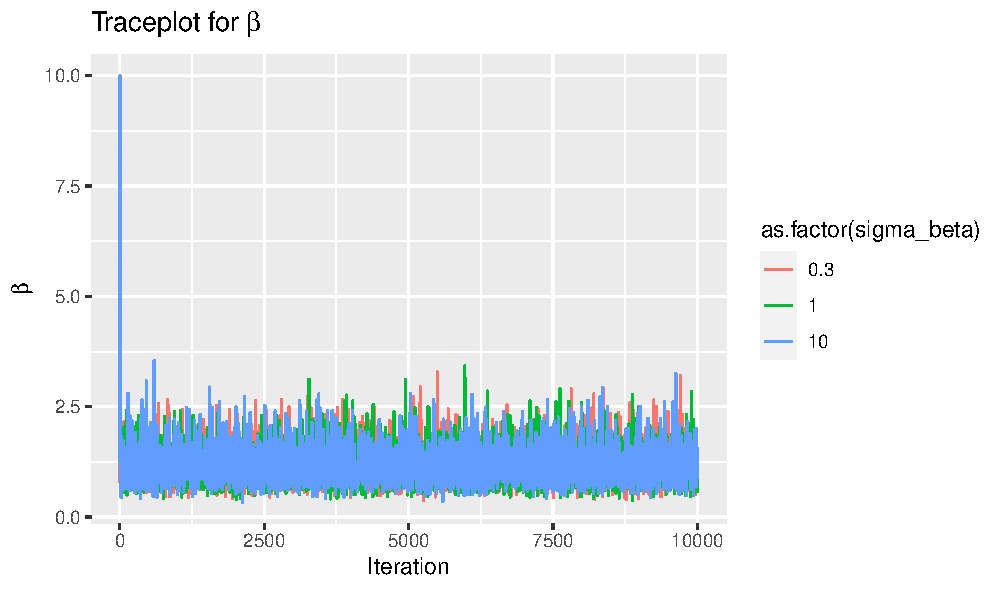
\includegraphics[width = \textwidth]{Images/tuning_beta_block_beta.pdf}
        \caption{$\beta$}

    \end{subfigure}
    \begin{subfigure}[b]{0.49\textwidth}
        \centering
        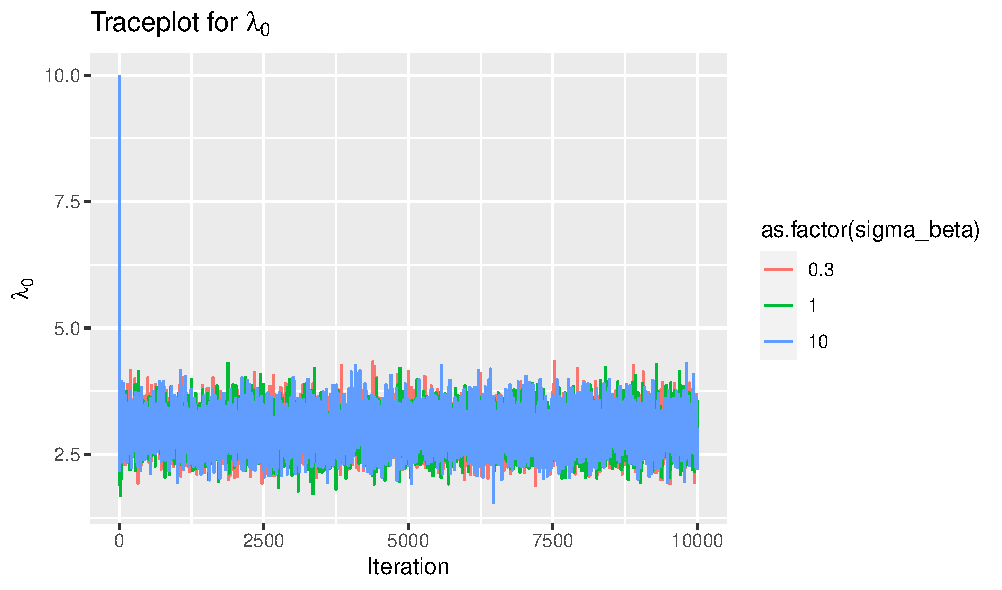
\includegraphics[width = \textwidth]{Images/tuning_lambda_0_block_beta.pdf}
        \caption{$\lambda_0$}

    \end{subfigure}
    \begin{subfigure}[b]{0.49\textwidth}
        \centering
        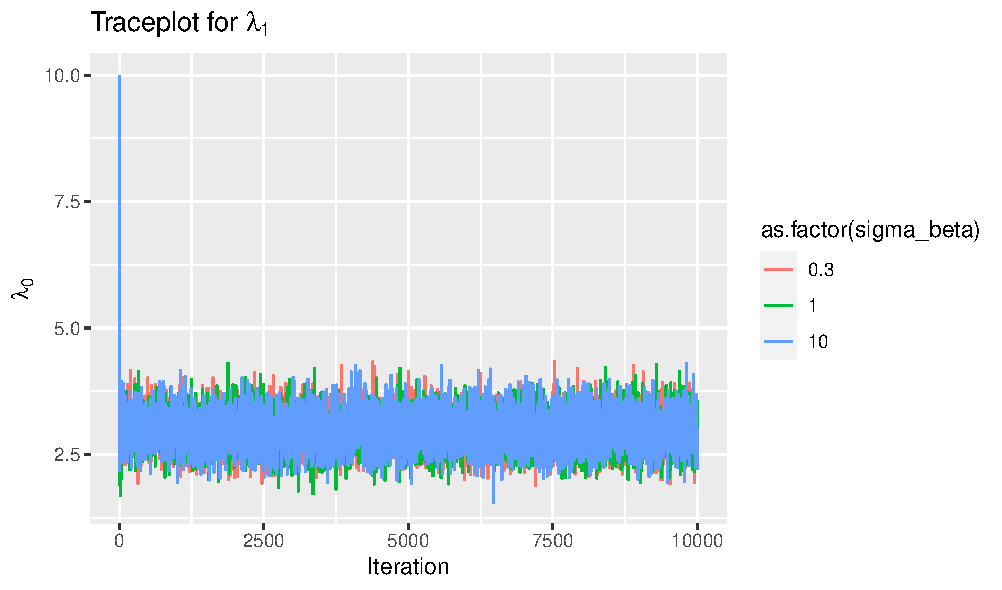
\includegraphics[width = \textwidth]{Images/tuning_lambda_1_block_beta.pdf}
        \caption{$\lambda_1$}

    \end{subfigure}
    \begin{subfigure}[b]{0.49\textwidth}
        \centering
        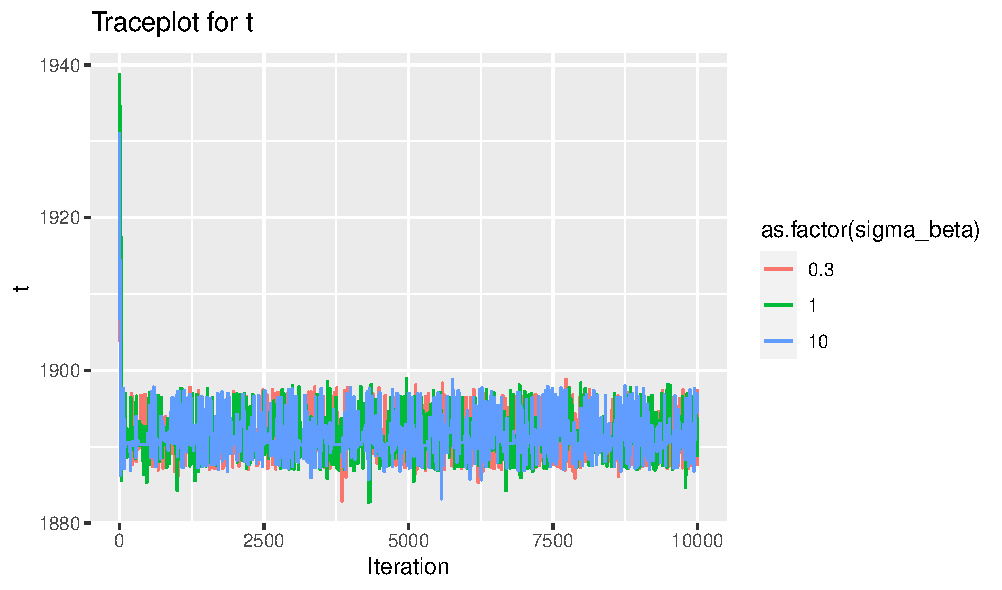
\includegraphics[width = \textwidth]{Images/tuning_t_block_beta.pdf}
        \caption{$t$}

    \end{subfigure}
     \caption{Trace plots for $n = 10000$ simulations with different values for tuning parameter $\sigma_{\beta}$ with the block MCMC algorithm. The initial values used are $\lambda_0 = 10, \lambda_1 = 5$, $t = 1931$. We test $\beta = (0.3, 1, 10)$ }
    \label{fig:tuning_beta_blockMH}
\end{figure}


 In Figure \ref{fig:tuning_t_blockMH} we have plotted the parameter $t$  for three different values of $\sigma_t$. It is not very clear from the figure but increasing the tuning parameter leads to a lower acceptance rate. We also sence how the steps taken by $t_1$ are smaller than the steps taken for $\sigma_t$ larger. It looks a bit like the chain does not mix so well for the lowest value of the tuning parameter. 
 
 In figure \ref{fig:tuning_beta_blockMH} we have plotted the trace plot of parameter $\beta$ for three different values of $\sigma_{\beta}$. Here the mixing of the chians is very good and the only difference we not is how many steps are accepted. 

We can use the simulated values of the parameters to estimate $\mathbf{E}[t_1|x], \mathbf{E}[\lambda_0|x]$ and $\mathbf{E}[\lambda_1|x]$. We do this by removing the burn-in period, and then finding the empirical means. 


\begin{table}[]
\centering
\begin{tabular}{lcccc}
                           & \textbf{t} & \textbf{$\lambda_0$} & \textbf{$\lambda_1$} & \textbf{$\beta$} \\ \hline
\textbf{Mean single site}  & 1891       & 3.084              & 0.9256             & 1.003         \\
\textbf{Mean block update} & 1891       & 3.014              & 0.9945             & 1.17         
\end{tabular}
\caption{Posterior means of $t$, $\lambda_0$, $\lambda_1$, and $\beta$}
\label{tab:mean}
\end{table}

We see from Table \ref{tab:mean} that the means using single site and block updating are quite similar. For $\beta$ it differs slightly. This could be due to computational errors. 

\begin{table}[]
\centering
\begin{tabular}{lc}
                      & \textbf{Cov($\lambda_1$, $\lambda_0$)} \\ \hline
\textbf{Single site}  & 0.00199                            \\
\textbf{Block update} & 0.01475                           
\end{tabular}
\caption{...}
\label{tab:cov}
\end{table}

From Table \ref{tab:cov} we see that the covariance is lower in the single site update than in the block update. This could be because in the block update either both are updated together with t or all rejected. This could mean that only "good" combinations of $\lambda_0$ and $\lambda_1$ are accepted. 


\todo[color = yellow]{Sett in posterior plotsene de ligger inder images. Prøv å lag fire plott med posterio til t for single og block ved siden av hverandre etc.. }


We see that the posterior densities look quite similar when using the single site versus the block updating. 





